% Déclaration du type de document (report, book, paper, etc...)
\documentclass[a4paper, 12pt]{paper} 
 
% Package pour avoir Latex en français
\usepackage[utf8]{inputenc}
\usepackage[T1]{fontenc}
 
% Quelques packages utiles
\usepackage{listings} % Pour afficher des listings de programmes
\usepackage{graphicx} % Pour afficher des figures
\usepackage{amsthm}   % Pour créer des théorèmes et des définitions
\usepackage{amsmath}
\usepackage{microtype} % Optical margins FTW
\usepackage{url}
\usepackage{booktabs} % Allows the use of \toprule, \midrule and \bottomrule in tables for horizontal lines
\usepackage[per-mode=symbol]{siunitx}
\usepackage{floatrow}
\usepackage{caption}
\usepackage{subcaption}
\usepackage{fullpage}
\usepackage{lipsum}



\author{Loïc Amez-Droz \and Florian Reinhard}
\title{Pinhole camera}

% Début du document
\begin{document}
\begin{titlepage}
\begin{center}
    \textsc{\LARGE École Polytechnique Fédérale de~Lausanne}\\[1.5cm] 
    {\huge \bfseries Optical Engineering: Multimode Fibre}\\[0.4cm] 
    \begin{tabular}{|p{5cm}|p{4cm}|}
        \hline
        Group & C-XX \\ \hline
        Students & Loïc \textsc{Amez-Droz} \newline Florian \textsc{Reinhard} \\ \hline
        Date of lecture & 13.03.2015 \\ \hline
        Date of final report return & 20.03.2015 \\ \hline
    \end{tabular}
\end{center}


\begin{abstract}
    \lipsum[3]
\end{abstract}
 
\vfill
\end{titlepage}

\section{Procedures and results}
\subsection{Imaging with a pinhole camera}

\begin{figure}[H]
    \centering
    \begin{subfigure}[t]{0.45\textwidth}
        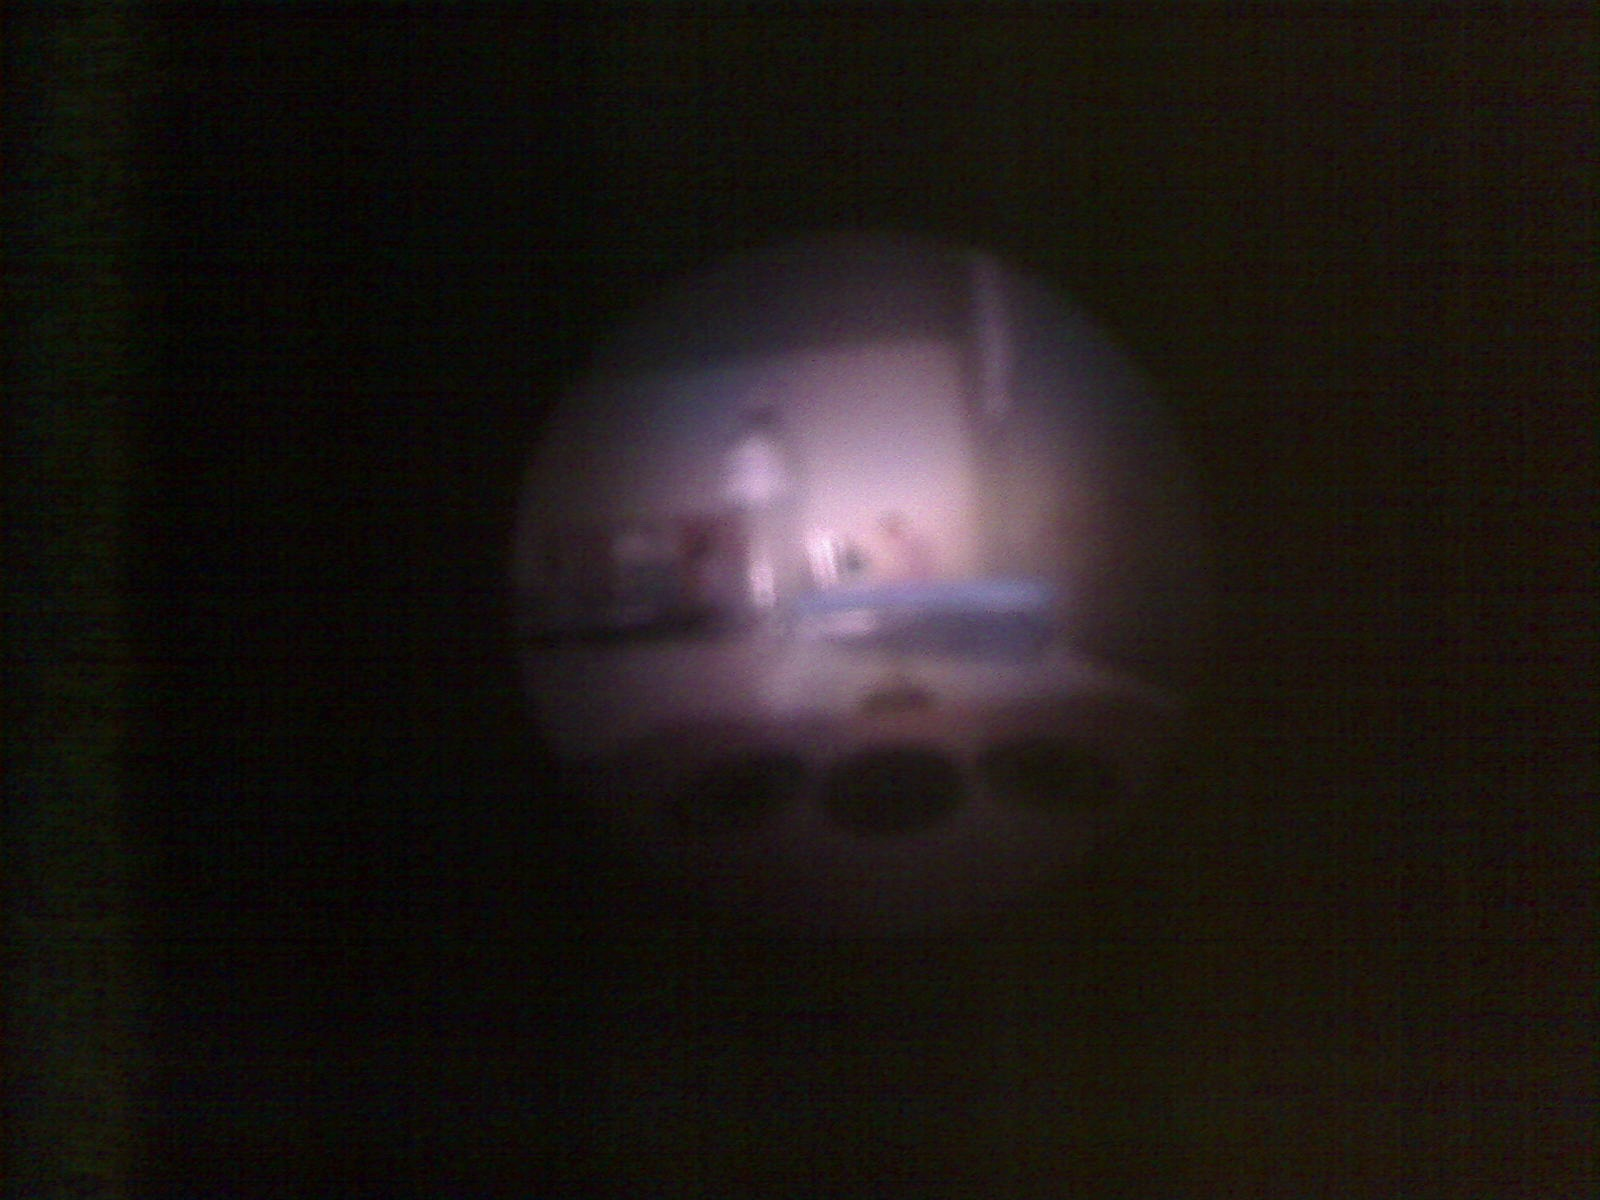
\includegraphics[width=\textwidth]{img/00mm}
        \caption{\SI{0.7}{\milli\meter}}
    \end{subfigure}
    \begin{subfigure}[t]{0.45\textwidth}
        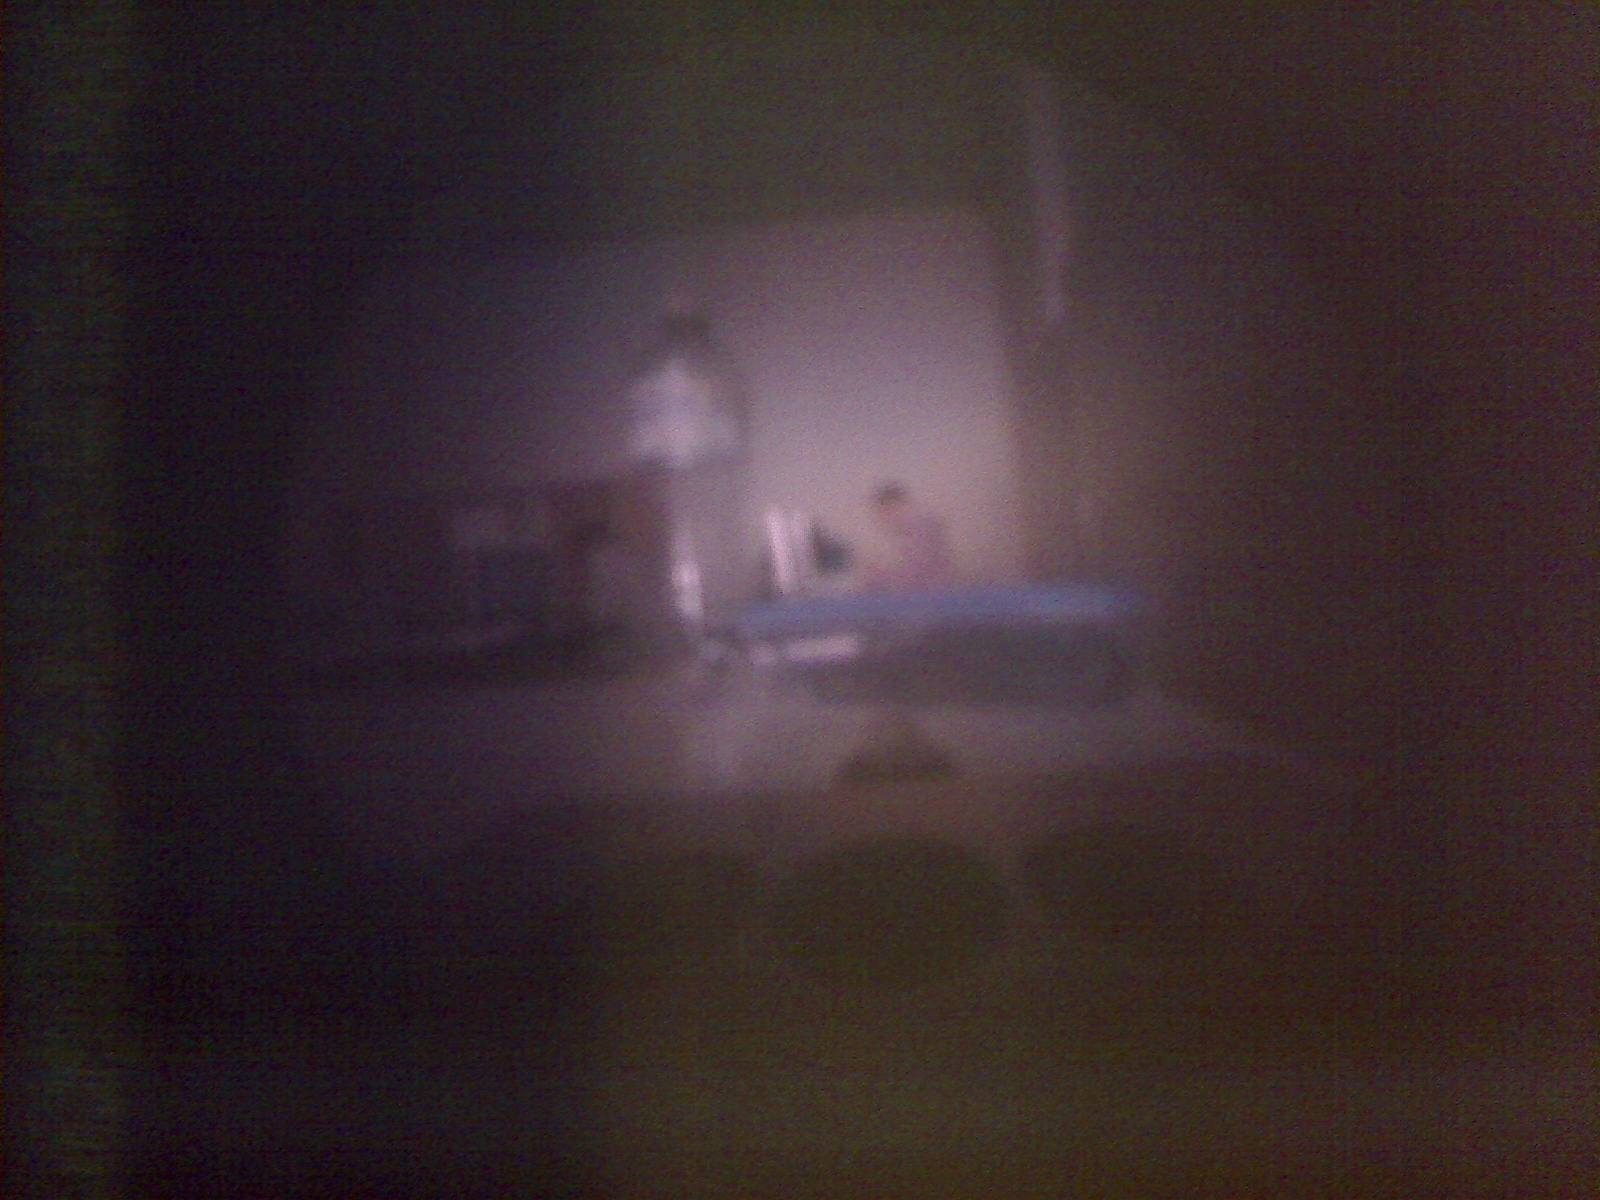
\includegraphics[width=\textwidth]{img/05mm}
        \caption{\SI{1.2}{\milli\meter}}
    \end{subfigure}
    \begin{subfigure}[t]{0.45\textwidth}
        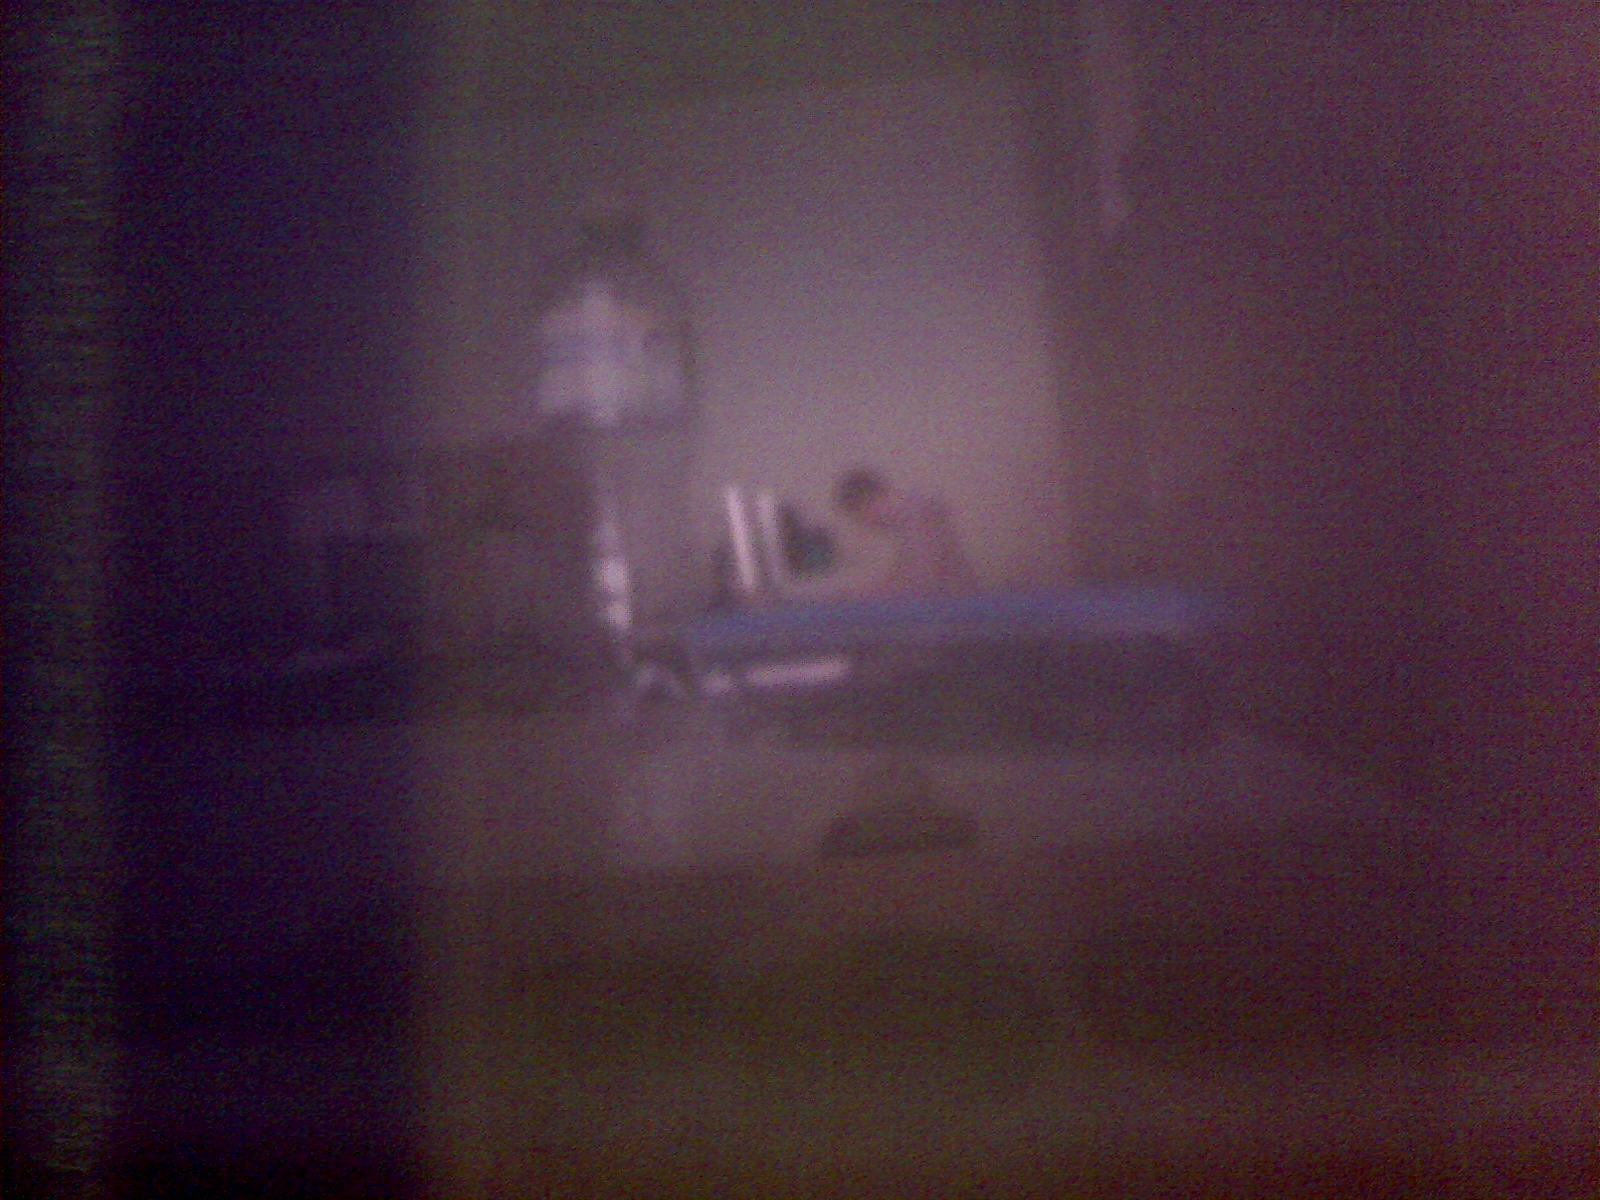
\includegraphics[width=\textwidth]{img/10mm}
        \caption{\SI{1.7}{\milli\meter}}
    \end{subfigure}
    \begin{subfigure}[t]{0.45\textwidth}
        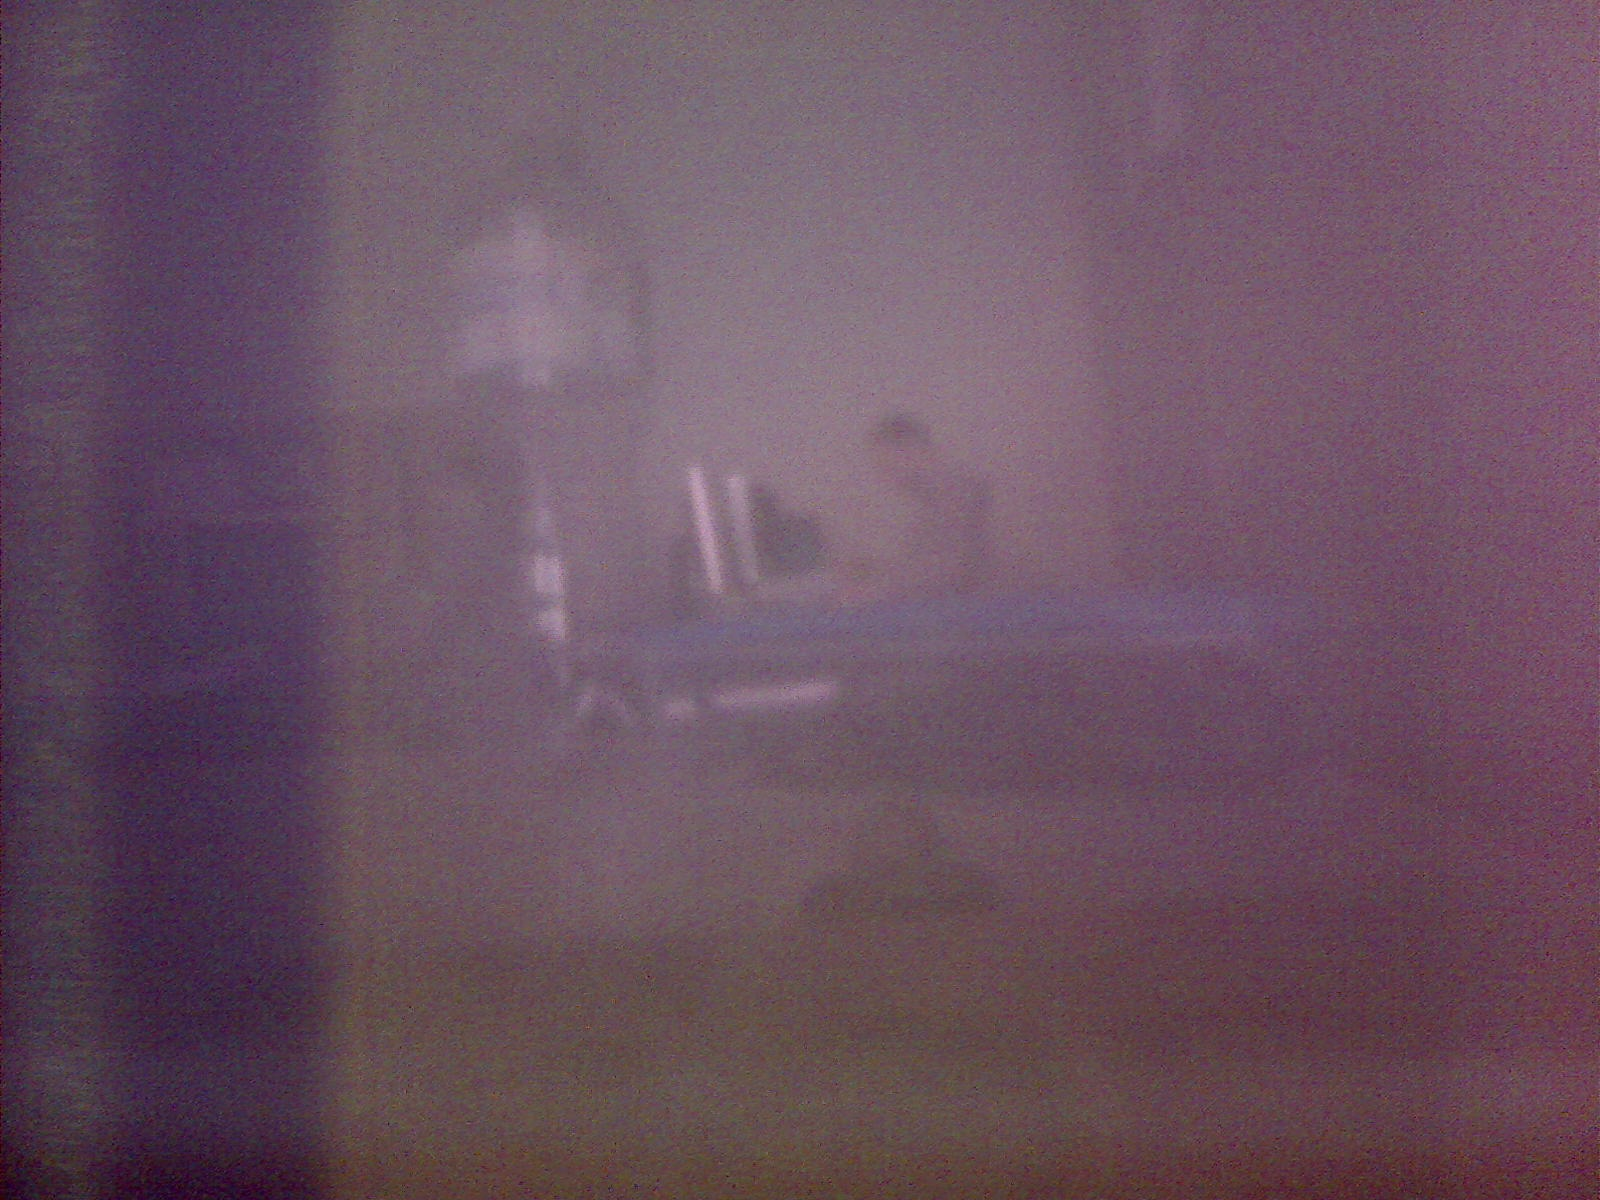
\includegraphics[width=\textwidth]{img/15mm}
        \caption{\SI{2.2}{\milli\meter}}
    \end{subfigure}
    \caption{Pinhole camera imaging with different distances of the pinhole from the camera sensor. With increasing distance, the image is magnified.
        Also, the \emph{f-number} increases and thus the field of depth.}
\label{fig:imaging}
\end{figure}

\subsection{Intensity distribution over the field}

The special intensity distribution of the pinhole camera can be compared with the $\cos^4 \theta$ function.
We expect to observe this with a pinhole camera with distance pinhole-detector approximately \SI{1.2}{\milli\meter}.

\begin{figure}[H]
    \centering
    \begin{subfigure}[t]{0.45\textwidth}
        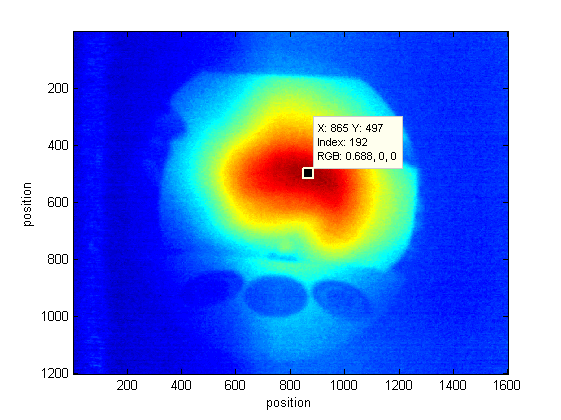
\includegraphics[width=\textwidth]{img/intensity_plot}
        \caption{Coloration according to intensity. The~maximum is at $x = 865$.}
    \end{subfigure}
    \begin{subfigure}[t]{0.45\textwidth}
        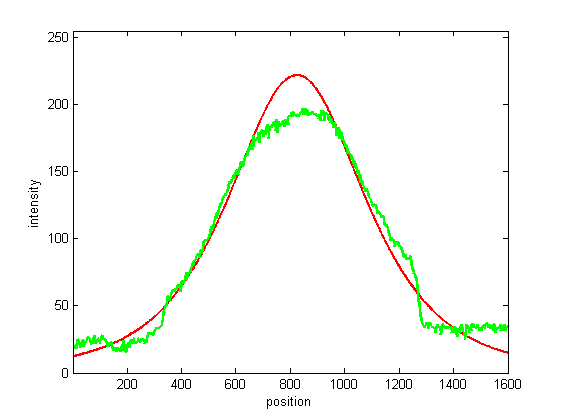
\includegraphics[width=\textwidth]{img/intensity_line_plot}
        \caption{Line plot at $y = 497$ (green) and $\cos^4 \theta$.}
    \end{subfigure}
\label{fig:intensity}
\end{figure}

The curve corresponds to the theoretical one although the presence of noise caused by offset.
The law derived from the emission irradiance $\cos^2 \theta$ dependence of a point situated at an angle $\theta$ from the optical axe.
Because the origin isn’t on the optical axe, the pinhole is perceived reduced; this creates a $\cos \theta$ dependence.
And the blot caused by the not parallel rays is bigger than the parallel rays one.
The combination of these effects creates a $\cos^4 \theta$ dependence. 

\subsection{MTF measurement with the basic method}



\begin{figure}[H]
    \centering
    \begin{subfigure}[t]{0.40\textwidth}
        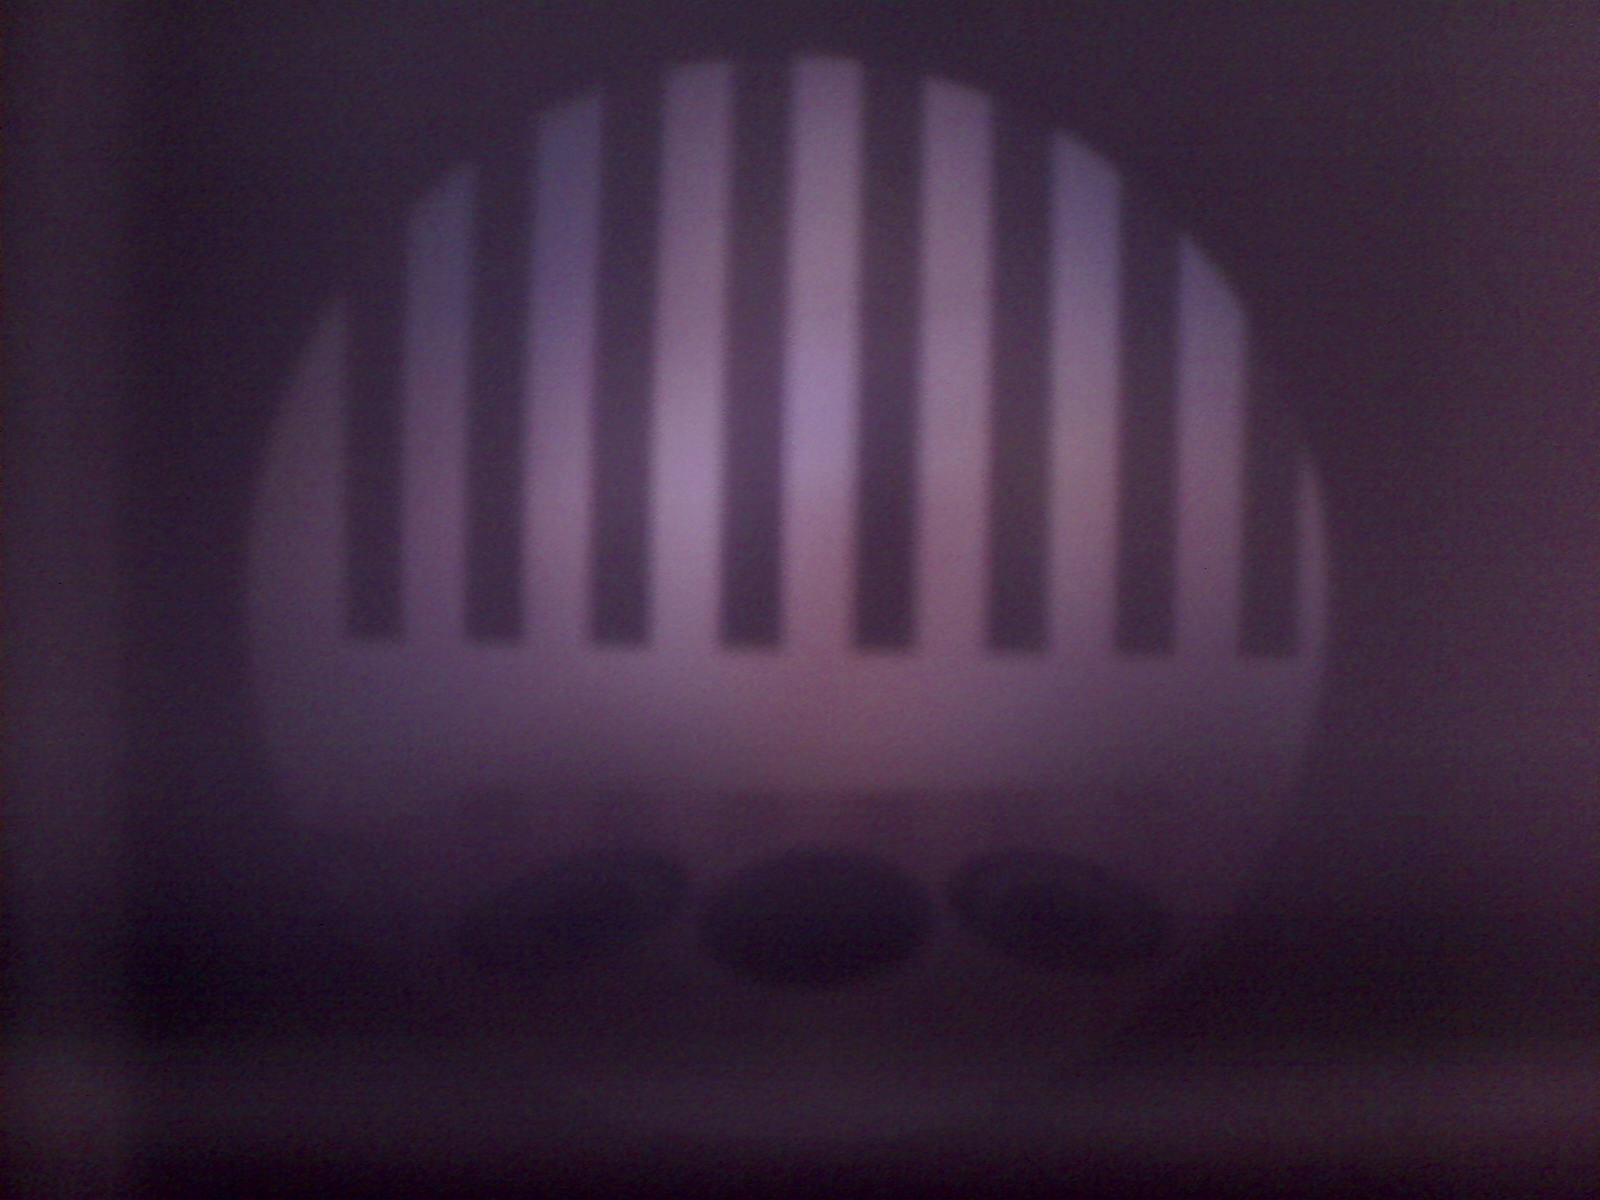
\includegraphics[width=\textwidth]{img/100}
        \caption{Max contrast.}
    \end{subfigure}
    \begin{subfigure}[t]{0.45\textwidth}
        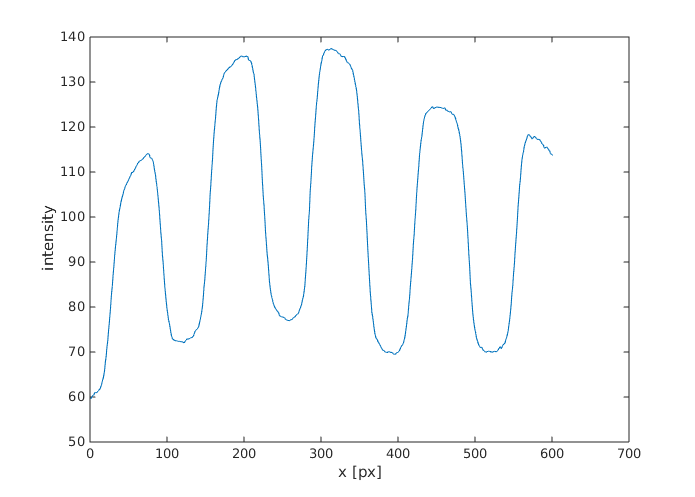
\includegraphics[width=\textwidth]{img/line_plot_100}
        \caption{Max contrast line plot.}
    \end{subfigure}
    \begin{subfigure}[t]{0.40\textwidth}
        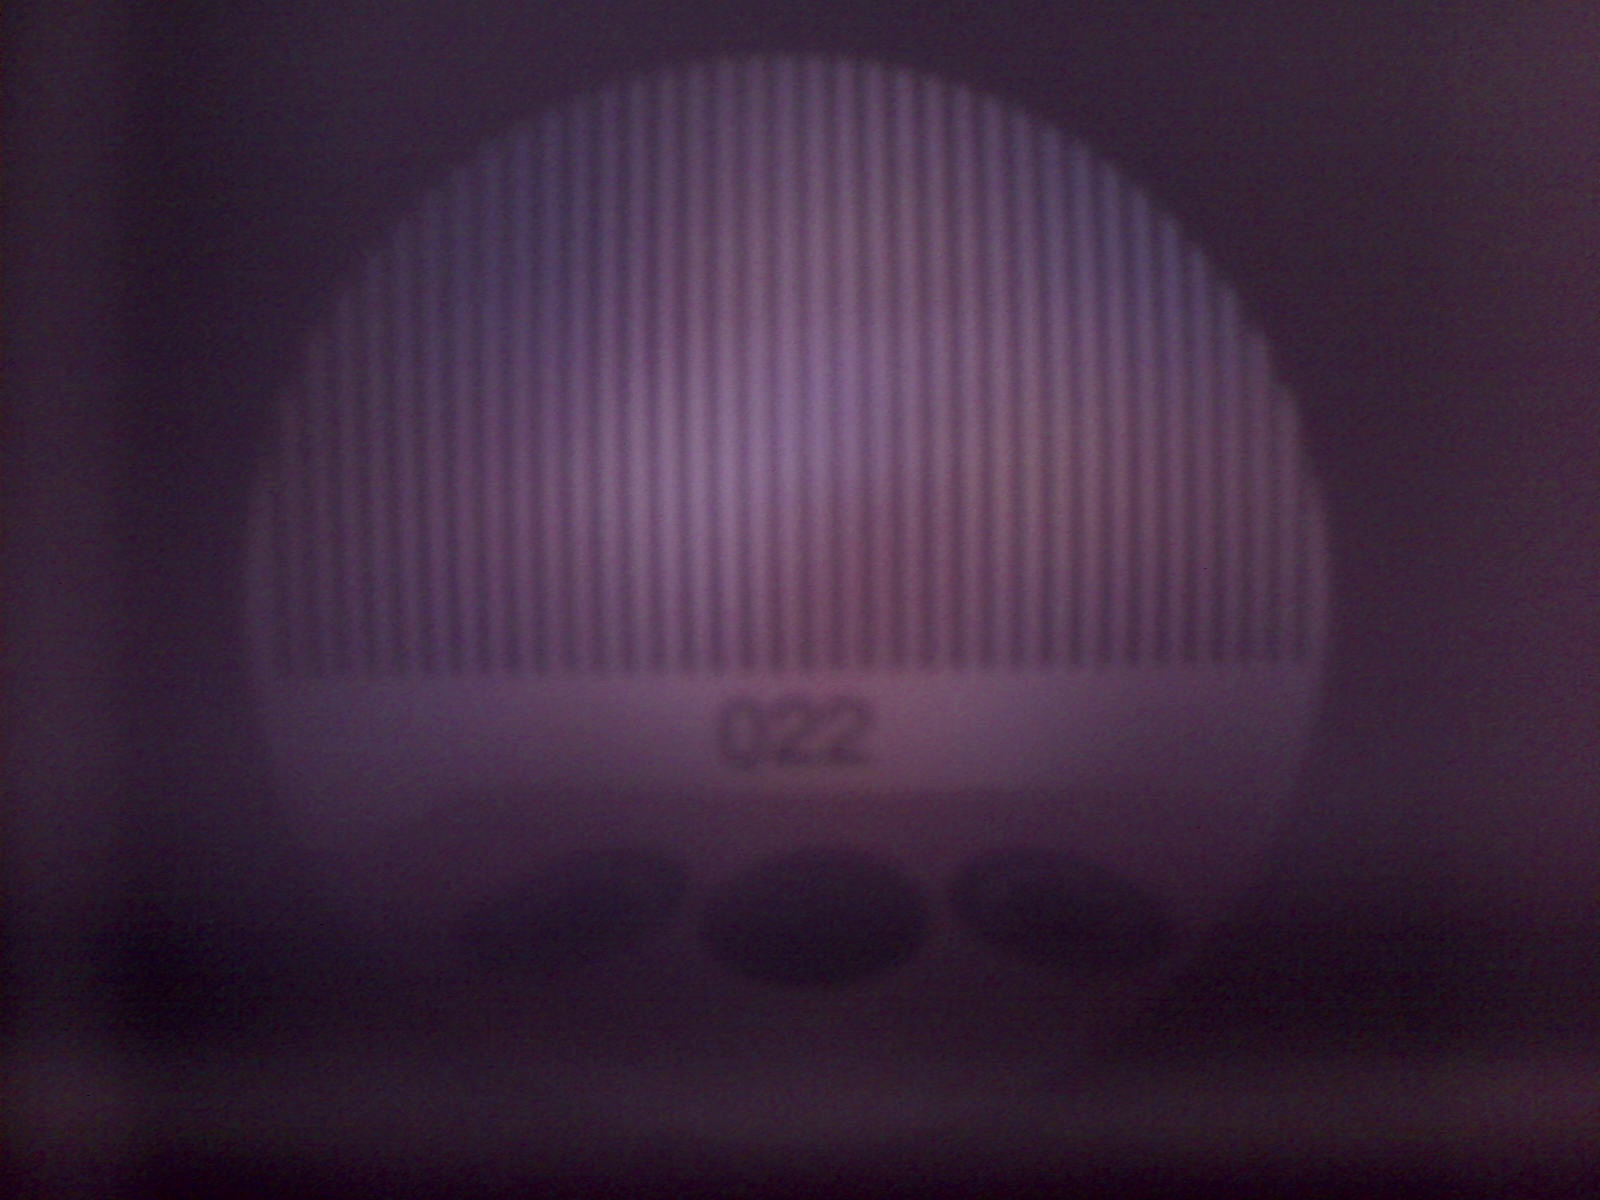
\includegraphics[width=\textwidth]{img/22}
        \caption{Medium contrast.}
    \end{subfigure}
    \begin{subfigure}[t]{0.45\textwidth}
        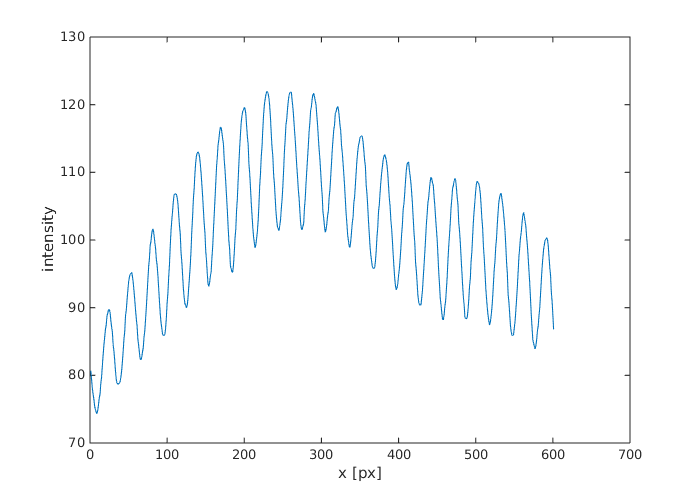
\includegraphics[width=\textwidth]{img/line_plot_22}
        \caption{Medium contrast line plot.}
    \end{subfigure}
    \begin{subfigure}[t]{0.40\textwidth}
        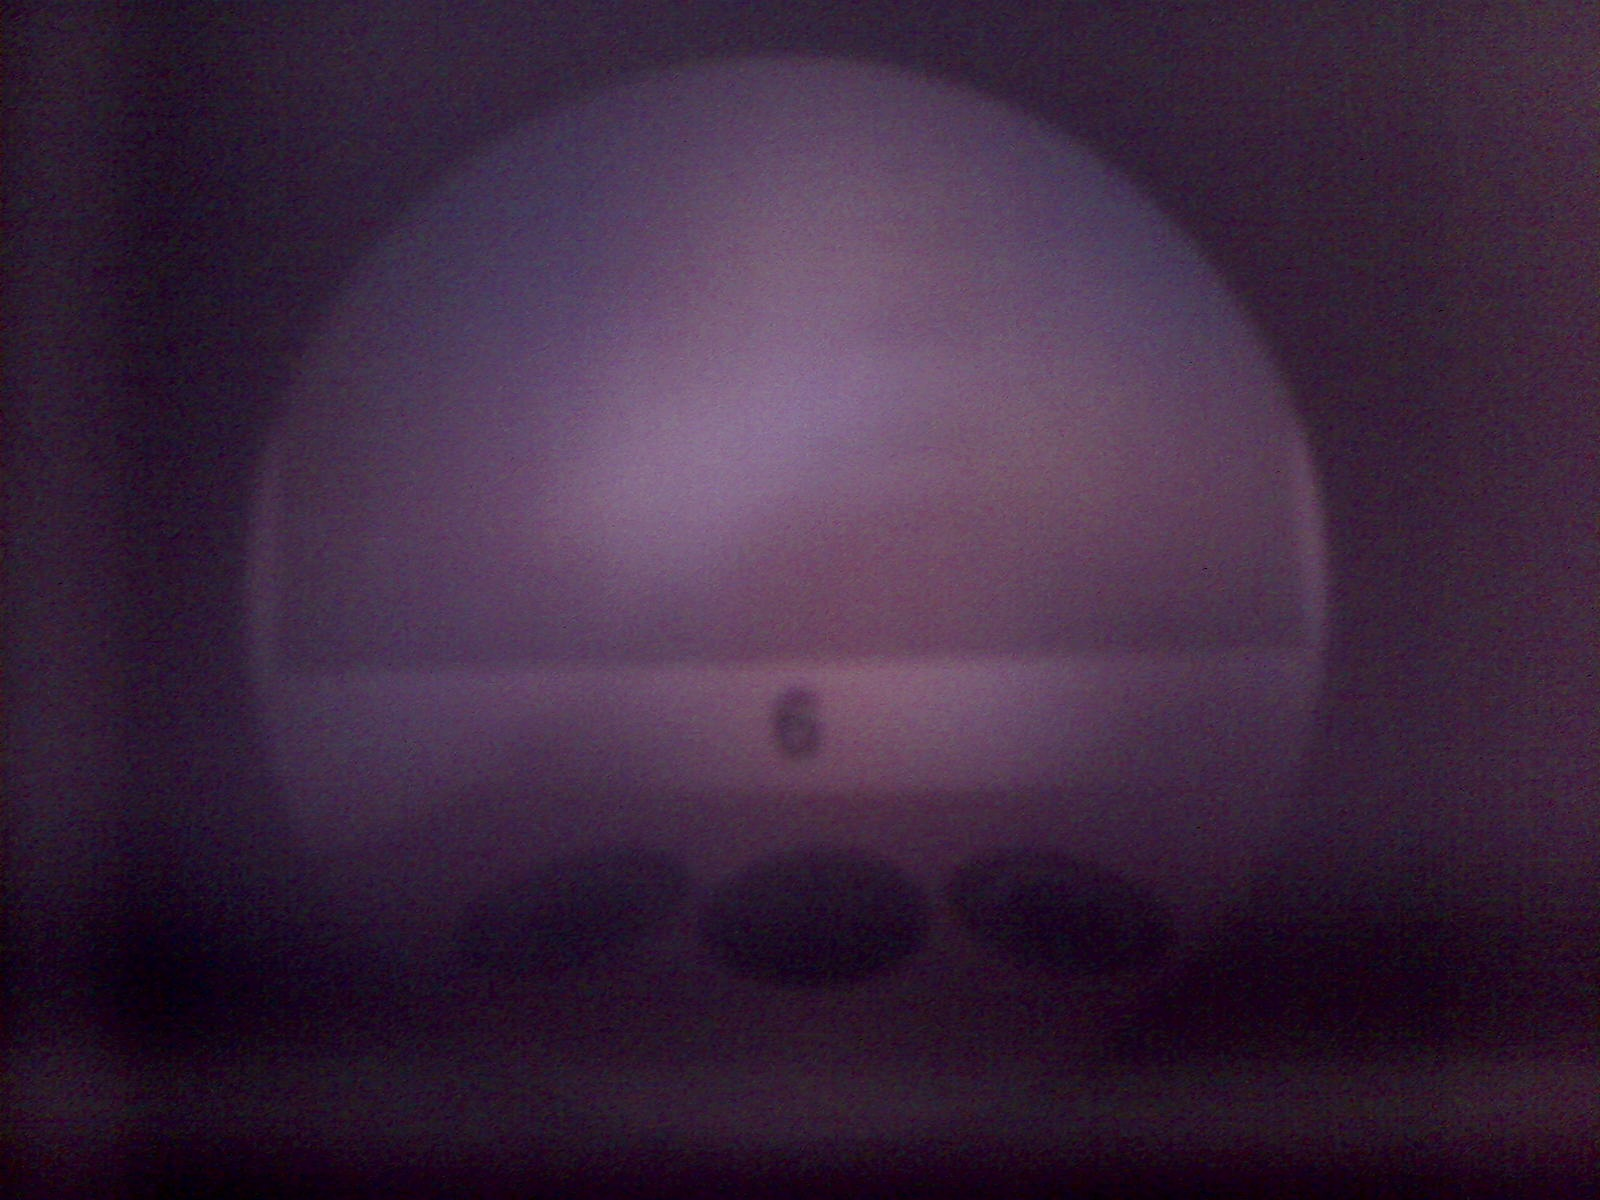
\includegraphics[width=\textwidth]{img/6}
        \caption{No contrast.}
    \end{subfigure}
    \begin{subfigure}[t]{0.45\textwidth}
        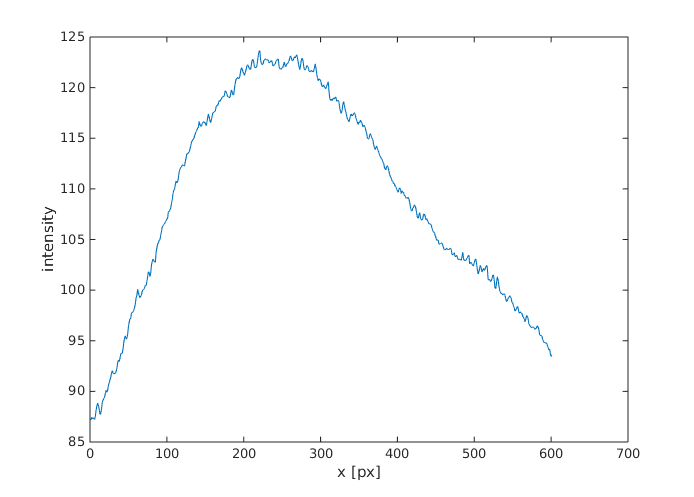
\includegraphics[width=\textwidth]{img/line_plot_6}
        \caption{No contrast line plot.}
    \end{subfigure}
    \caption{Typical pictures and their line plots.}
\label{fig:MTF}
\end{figure}


\begin{figure}[H]
    \centering
    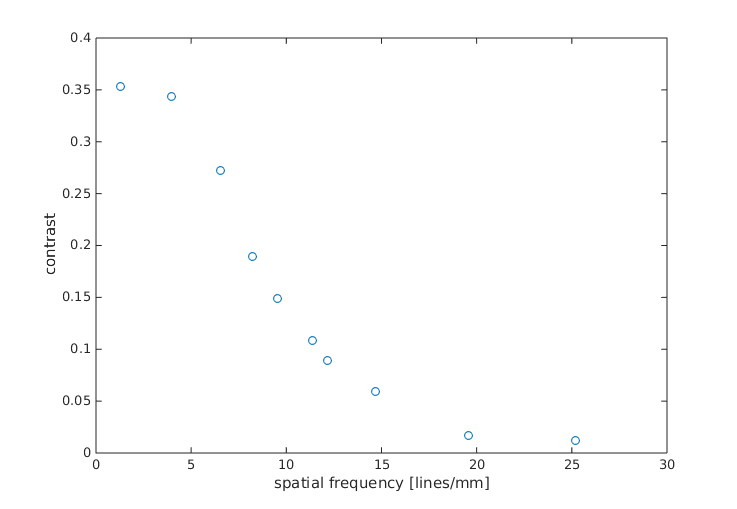
\includegraphics[width=0.8\textwidth]{img/contrast}
    \caption{Contrast in relation to spatial frequency.}
\label{fig:contrast}
\end{figure}


Noise seemed to dominate for spatial frequencies above $\nu_c = 35 \left[ \frac{\mbox{lines}}{\mbox{mm}} \right]$.
With a pinhole diameter $d = \SI{0.1}{\milli\meter}$ and a focal length of about $f = \SI{1.3}{\milli\meter}$, we calculate $\mbox{F\#} = \frac{f}{d} = 13$, which implies a theoretical cut-off frequency of $\nu_c = \frac{2000}{\mbox{F\#}} = 154 \left[ \frac{\mbox{lines}}{\mbox{mm}} \right]$. 

This discrepancy can be explained by the fact that the distance from the pinhole to the sensor wasn't optimal (equation~\ref{equ:distance}), because we didn't want that much of a magnification.

\begin{equation}
    d_2 \approx \frac{D^2}{4 \lambda} = \SI{5}{\milli\meter}
    \label{equ:distance}
\end{equation}

\subsection{Example from the Web}

\begin{figure}[H]
    \centering
    \begin{subfigure}[t]{0.4\textwidth}
        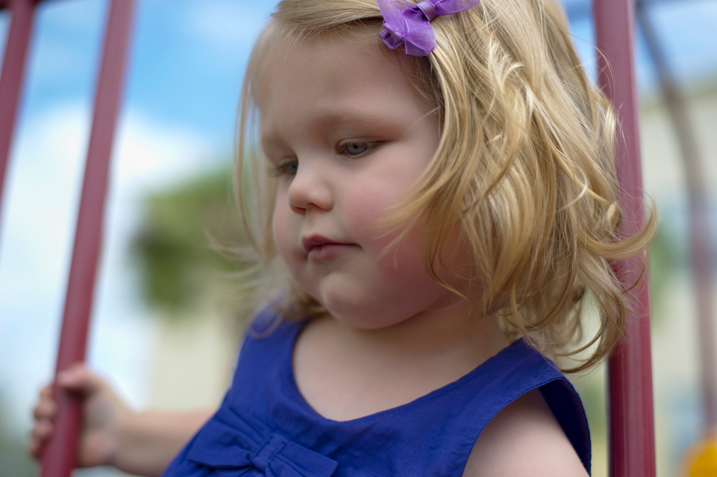
\includegraphics[width=\textwidth]{img/kid}
    \end{subfigure}
    \begin{subfigure}[t]{0.3\textwidth}
        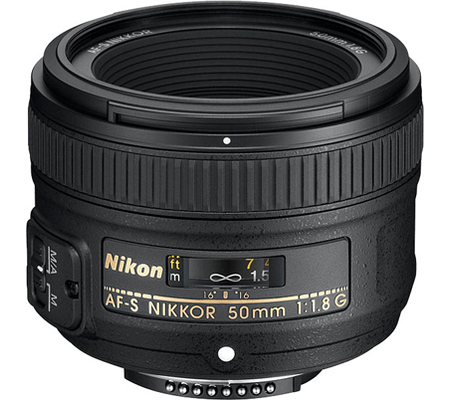
\includegraphics[width=\textwidth]{img/objective}
    \end{subfigure}
\label{fig:nikon}
\end{figure}

\begin{figure}[H]
    \centering
    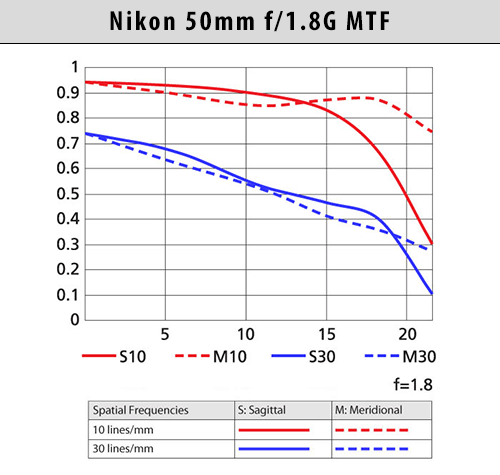
\includegraphics[width=0.6\textwidth]{img/nikon_mtf}
    \caption{The vertical axis represents the contrast/resolution (0-100\%) and the horizontal the distance from center to corner.}
\label{fig:nikon_MTF}
\end{figure}

We can see that the contrast is pretty good for both sagittal and meridional lines in the center and middle of the frame at the maximum aperture.
The resolution gradually decreases from the center to extreme corners.
There is almost no sign of wavy field curvature (no pikes in both curves).
The sagittal and meridional lines do not differ much for the $30 \left[ \frac{\mbox{lines}}{\mbox{mm}} \right]$ resolution, which means that astigmatism and lateral chromatic aberration isn’t well pronounced.

The picture comes from the Nikon website.

\section{Discussion and conclusions}

Comparing our pinhole camera to what an objective with lenses can do, we see that it is very much limited it what it can resolve; but it's an alternative for applications where low cost is important.
Also, the perceived cut-off frequency is much smaller than the pinhole's theoretical value.

\end{document}
